\clearpage

\section {Sensitivity with new Asimov data sets for Run 1-7c statistic.}
\label{sec:sensi_new_asimov_run17c}

Sensitivity studies for various values of true $\delta_{CP}$ were performed to give some context to our data constraint on $\delta_{CP}$. New Asimov data sets C, D and E are defined in \cref{tab:osc_params_joint_asimov} .
The effect of the true value of $\delta_{CP}$ was studied in the $\sin^2 \theta_{13}$ Vs $\delta_{CP}$, with and without the reactor constraint, and 1D $\delta_{CP}$ parameter spaces. The results are shown in \cref{fig:validation_sensi_2d_reactors_cde,fig:validation_sensi_dcp_cde}. Fits to Asimov data set C and D have similar results 
to Asimov data set B but provide slightly stronger constraint due to the additional events in the appearance samples due to more maximal disappearance. The fit to Asimov data set E is similar to that to Asimov data set A, both provide similar constraints on $\delta_{CP}$ however the more CP violating data set (E) naturally provides a stronger constraint.

\begin{figure*}[htb]
\center
%
\includegraphics[width=0.9\textwidth]{./images/missing_plot-eps-converted-to.pdf}
%
\includegraphics[width=0.9\textwidth]{./images/missing_plot-eps-converted-to.pdf}
%
\includegraphics[width=0.9\textwidth]{./images/missing_plot-eps-converted-to.pdf}
%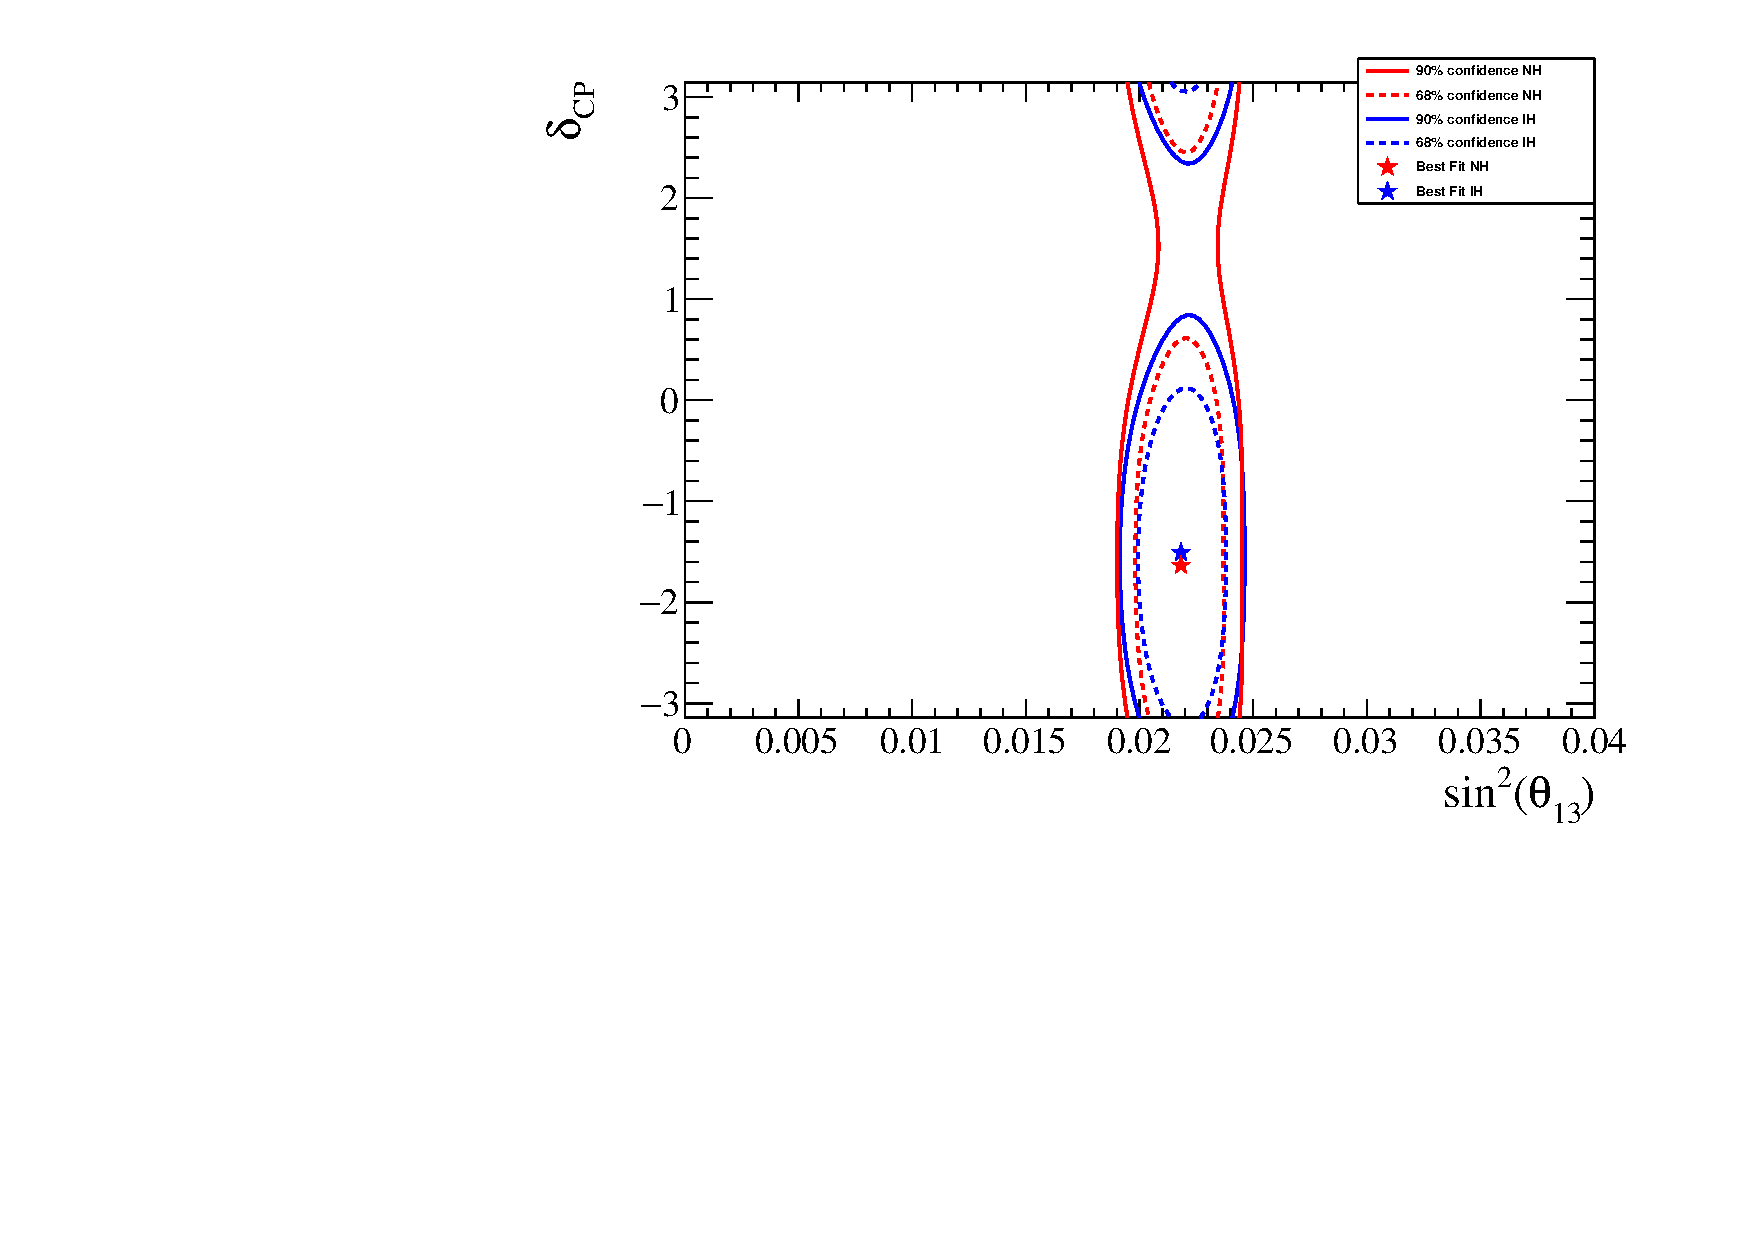
\includegraphics[width=0.9\textwidth]{./joint_plots/sensitivities/2D/cp13_reactor/cp13_reactor_A.pdf}
%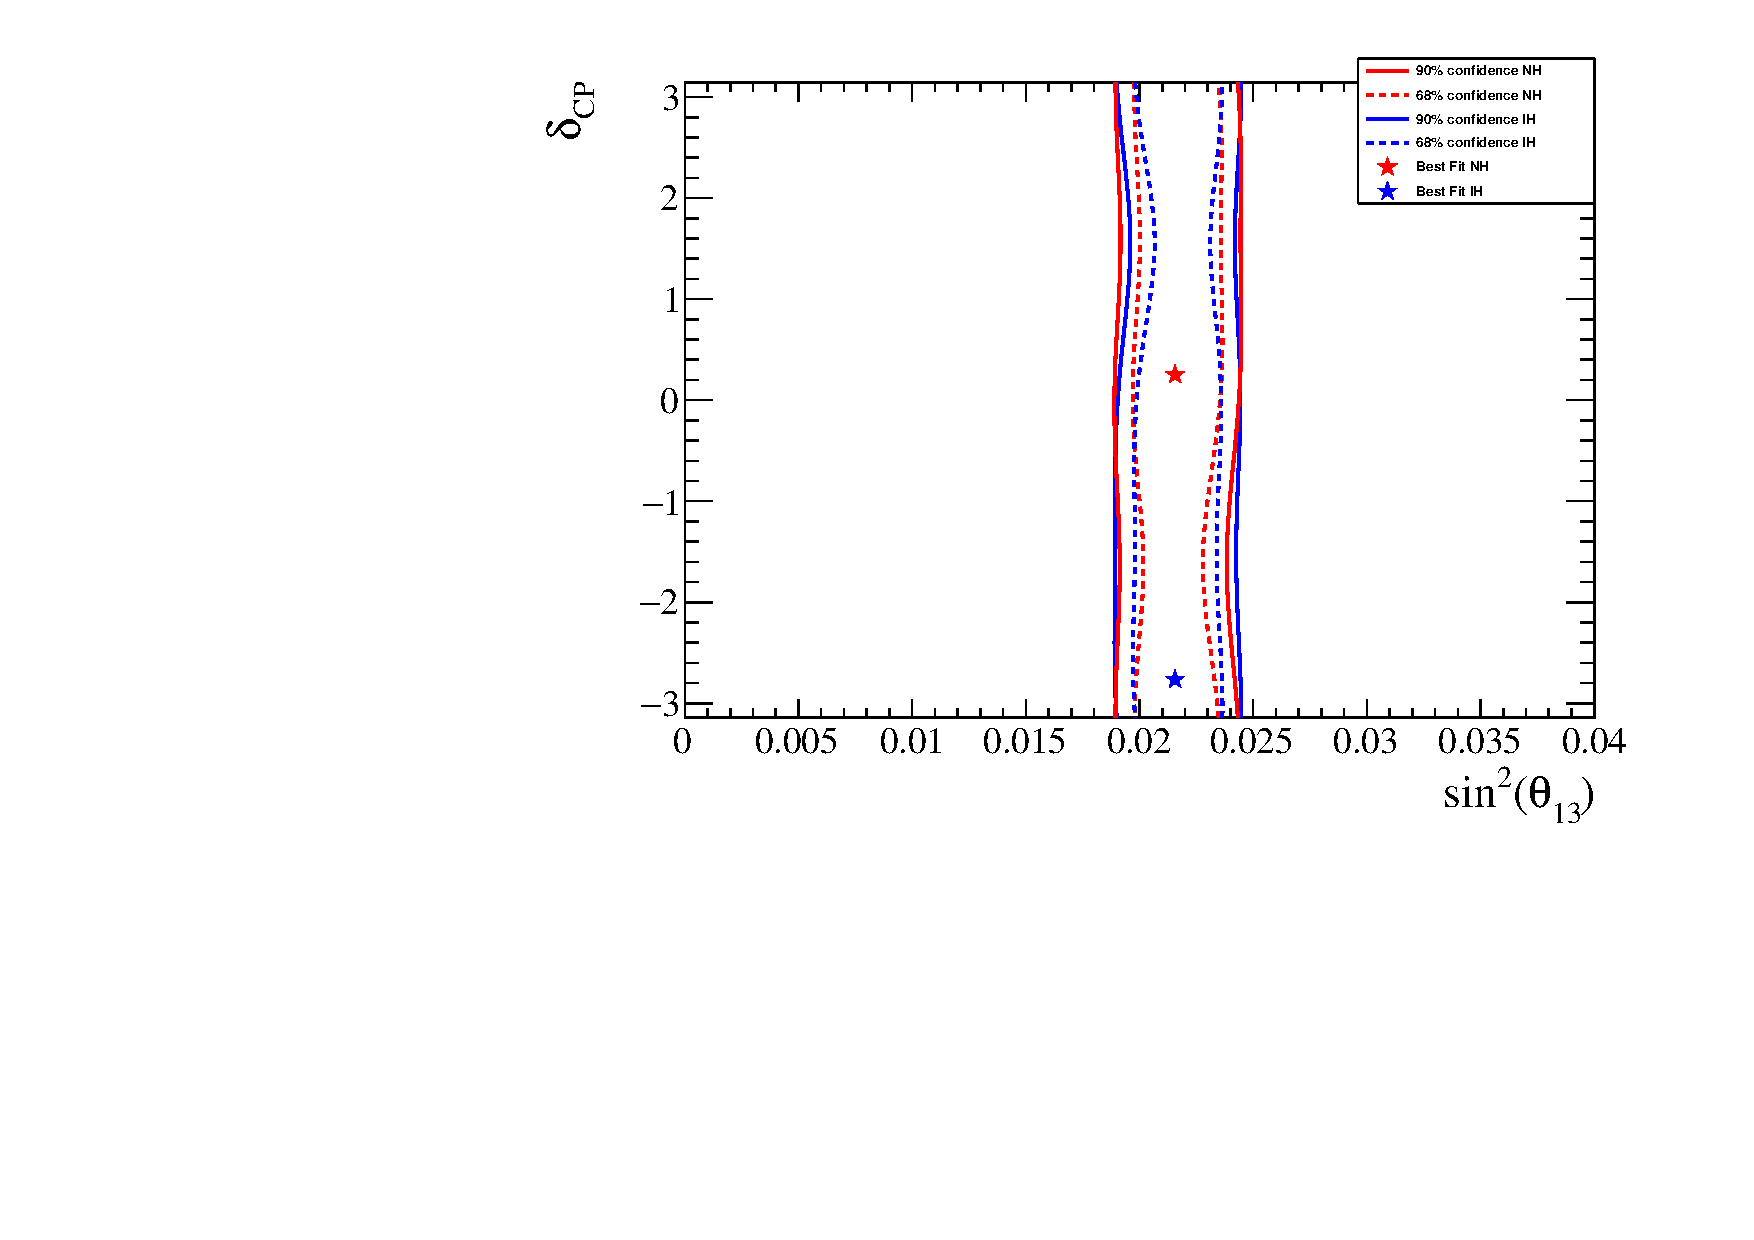
\includegraphics[width=0.9\textwidth]{./joint_plots/sensitivities/2D/cp13_reactor/cp13_reactor_B.pdf}
%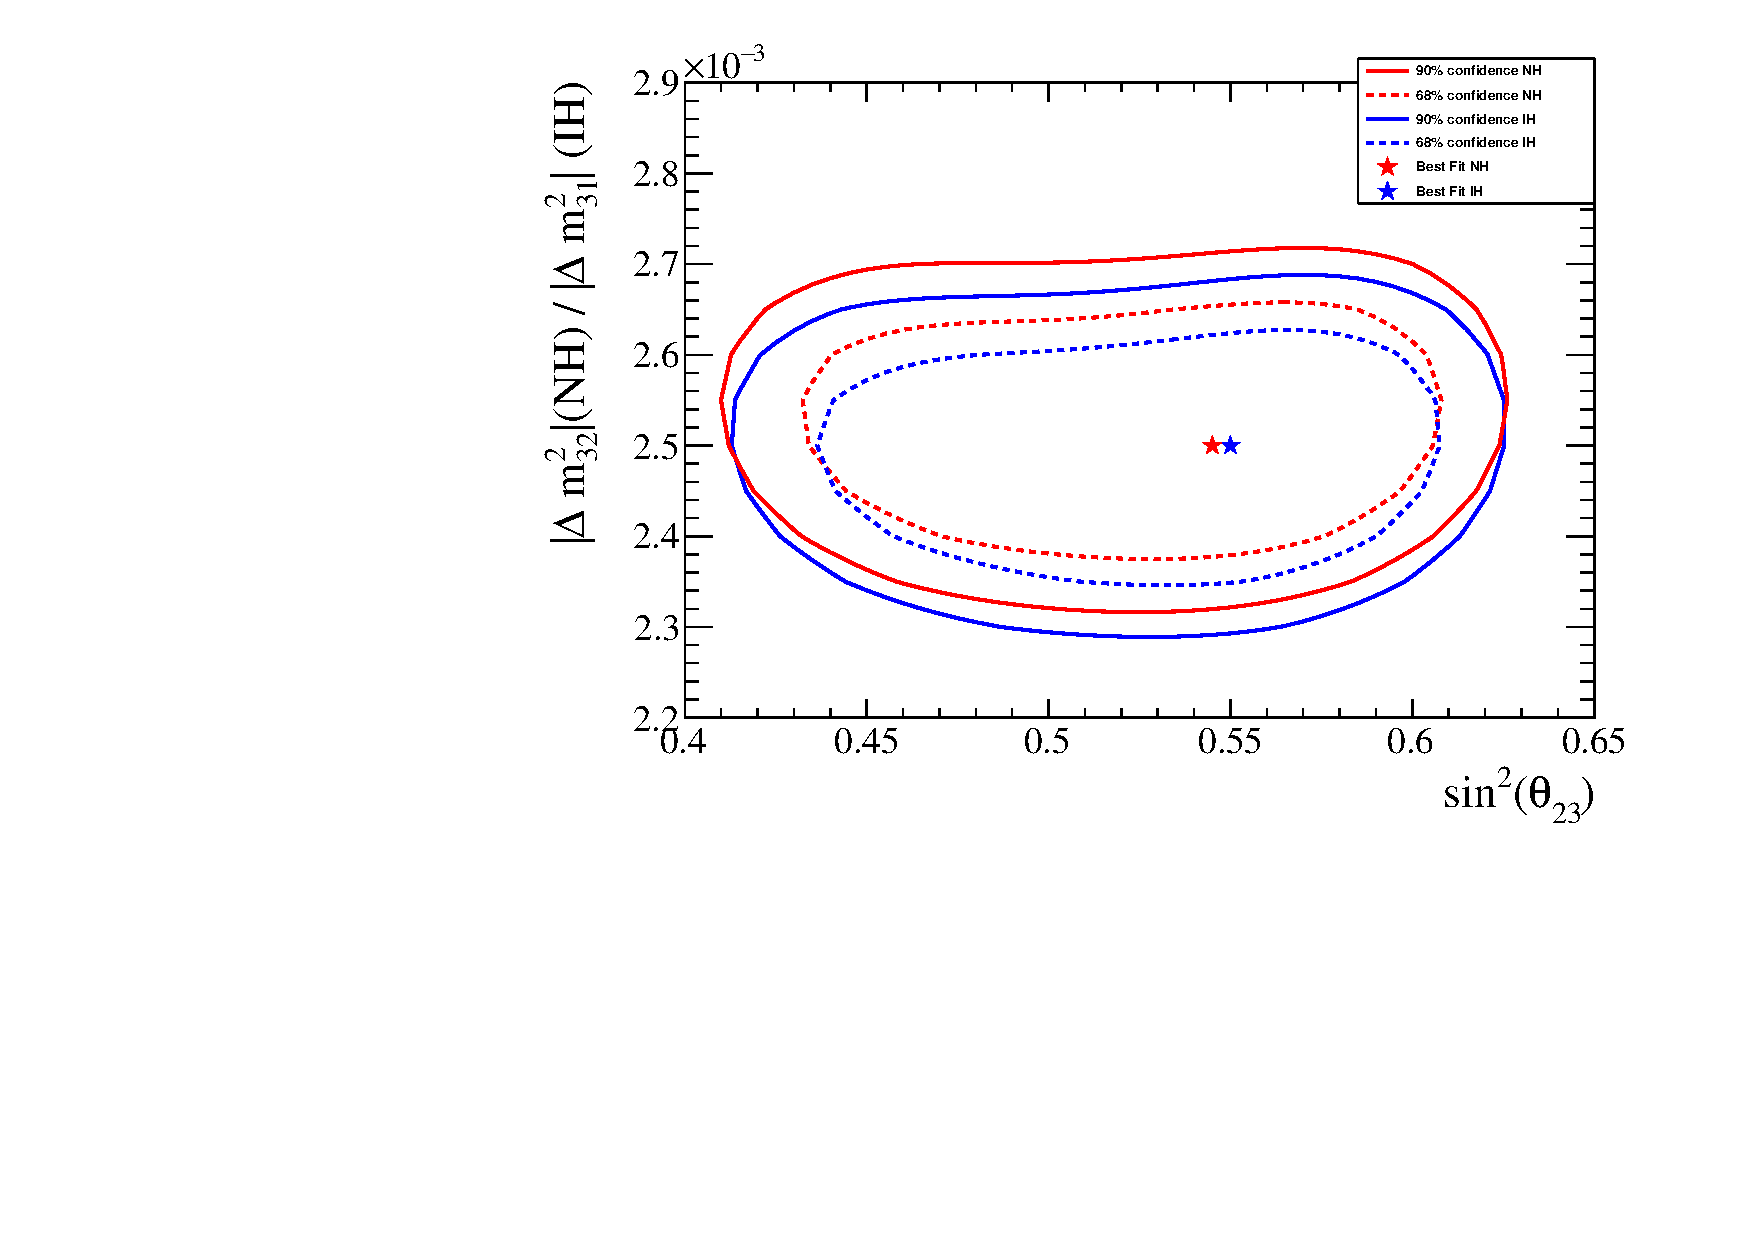
\includegraphics[width=0.9\textwidth]{./joint_plots/sensitivities/2D/ss23dmsq/ss23dmsq_A.pdf}
%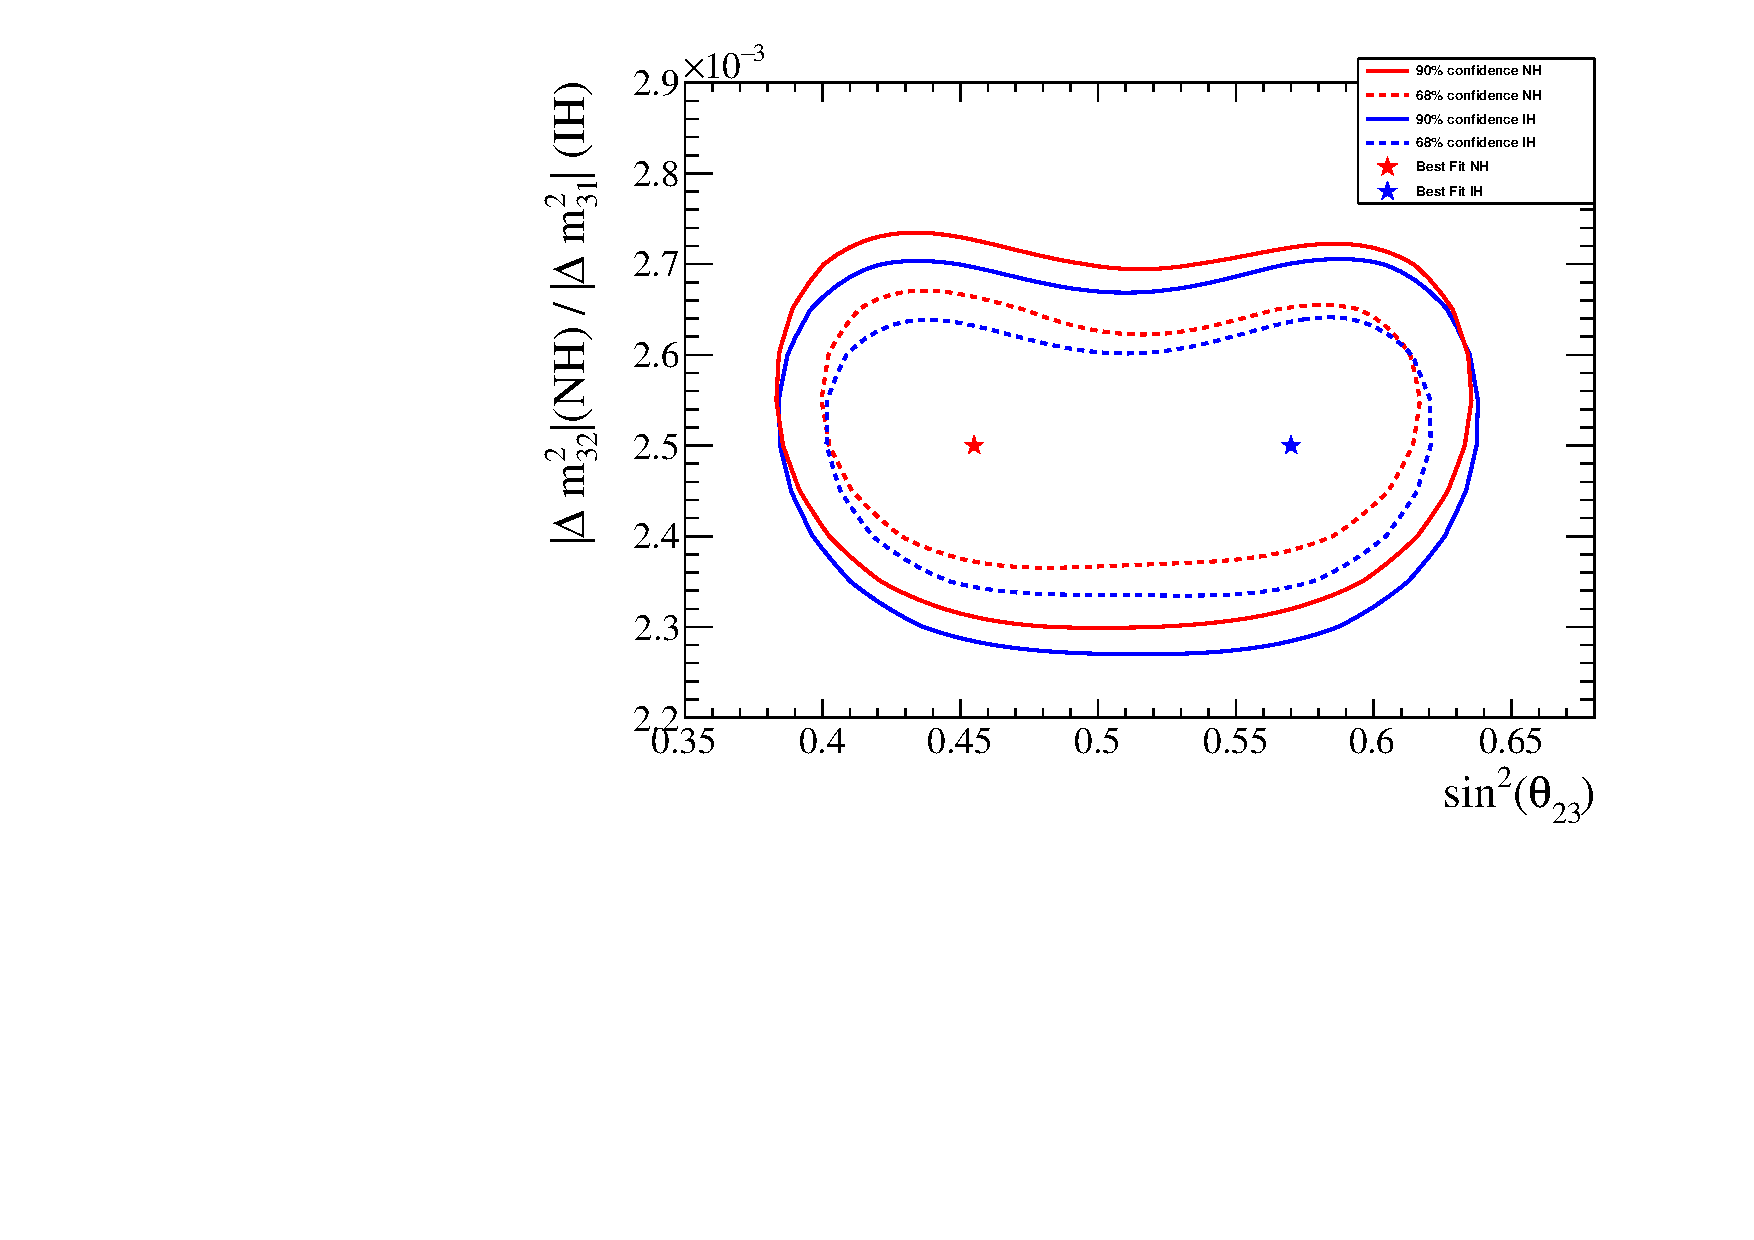
\includegraphics[width=0.9\textwidth]{./joint_plots/sensitivities/2D/ss23dmsq/ss23dmsq_B.pdf}
\begin{subfigure}[b]{0.49\textwidth}
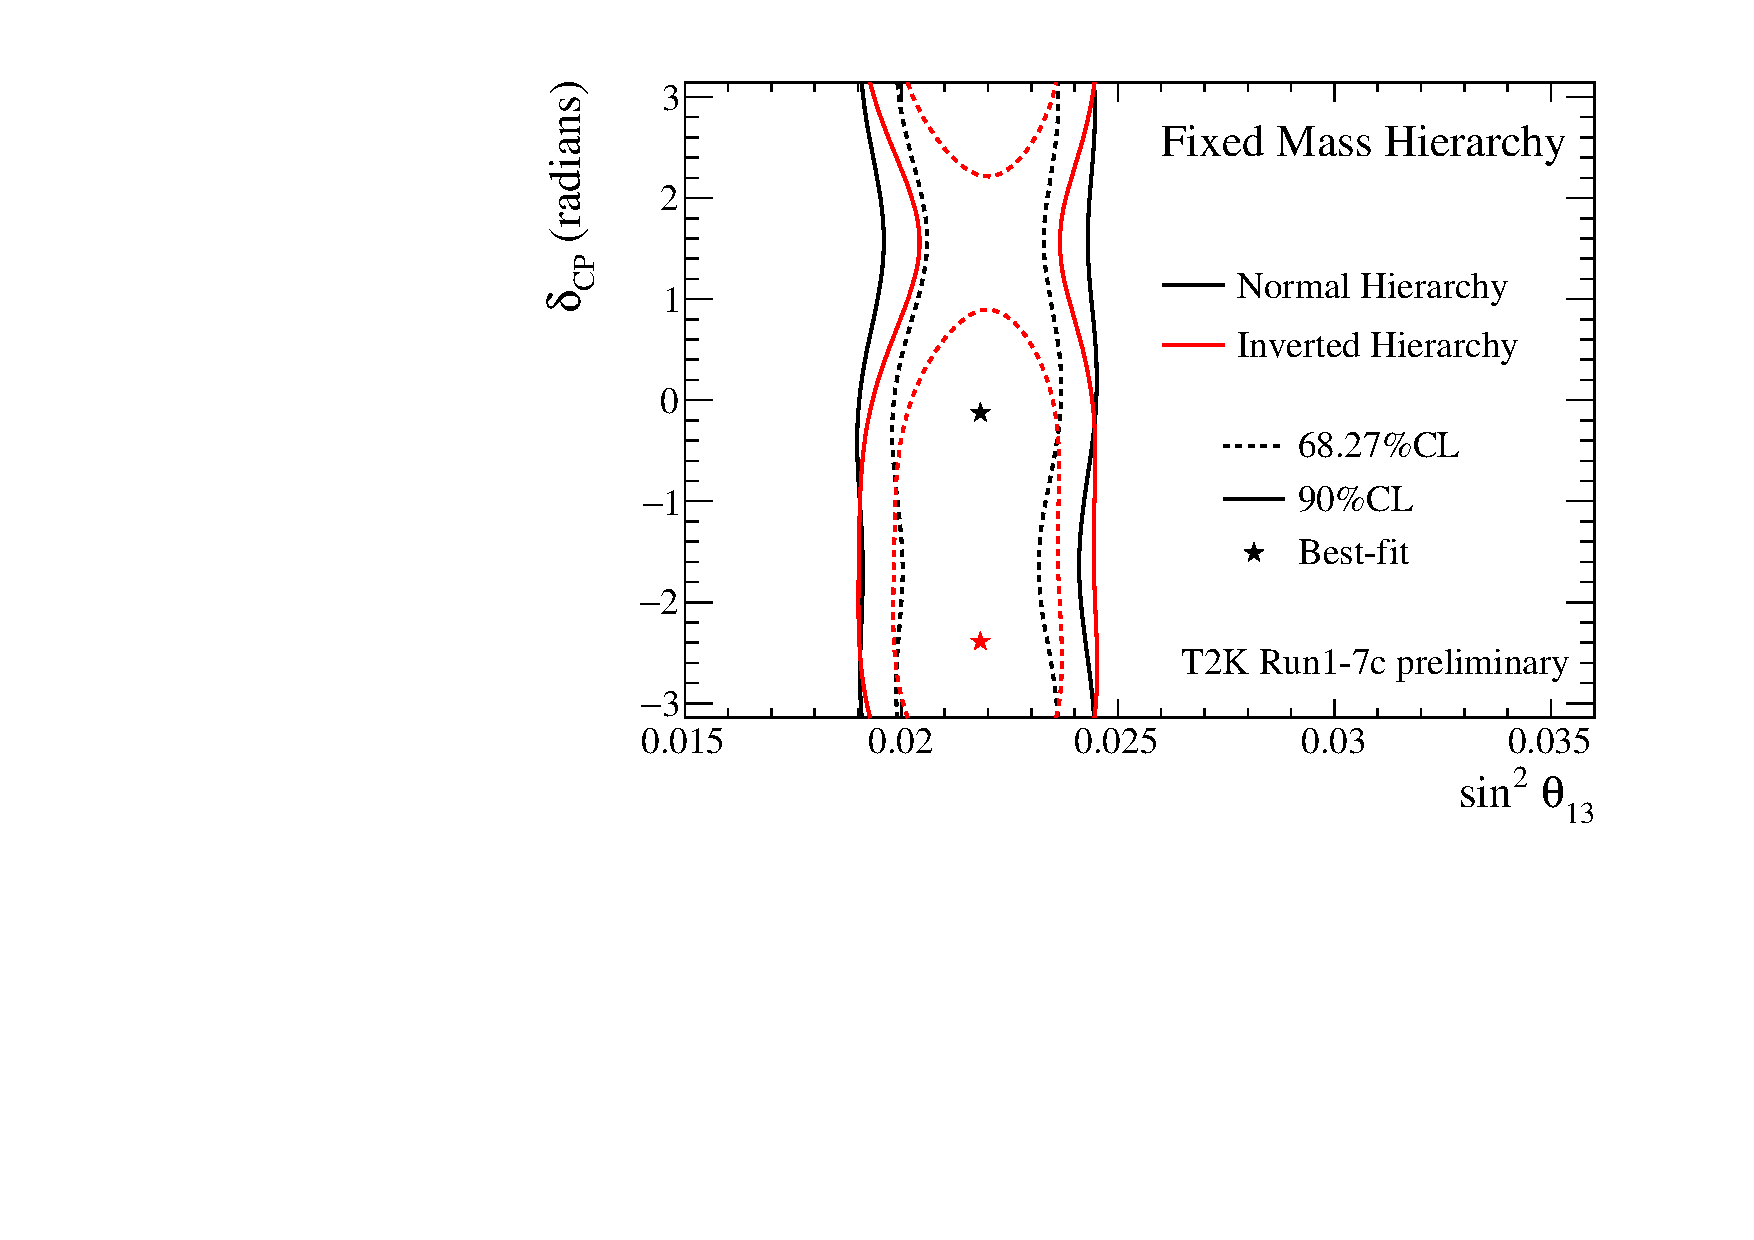
\includegraphics[width=0.9\textwidth]{./joint_plots/sensitivities/CDE/C_dcp_ss13_reactor.pdf}
\caption{Asimov C: $\sin^2 \theta_{13}$ Vs $\delta_{CP}$. Reactor constraint.}
\end{subfigure}
\begin{subfigure}[b]{0.49\textwidth}
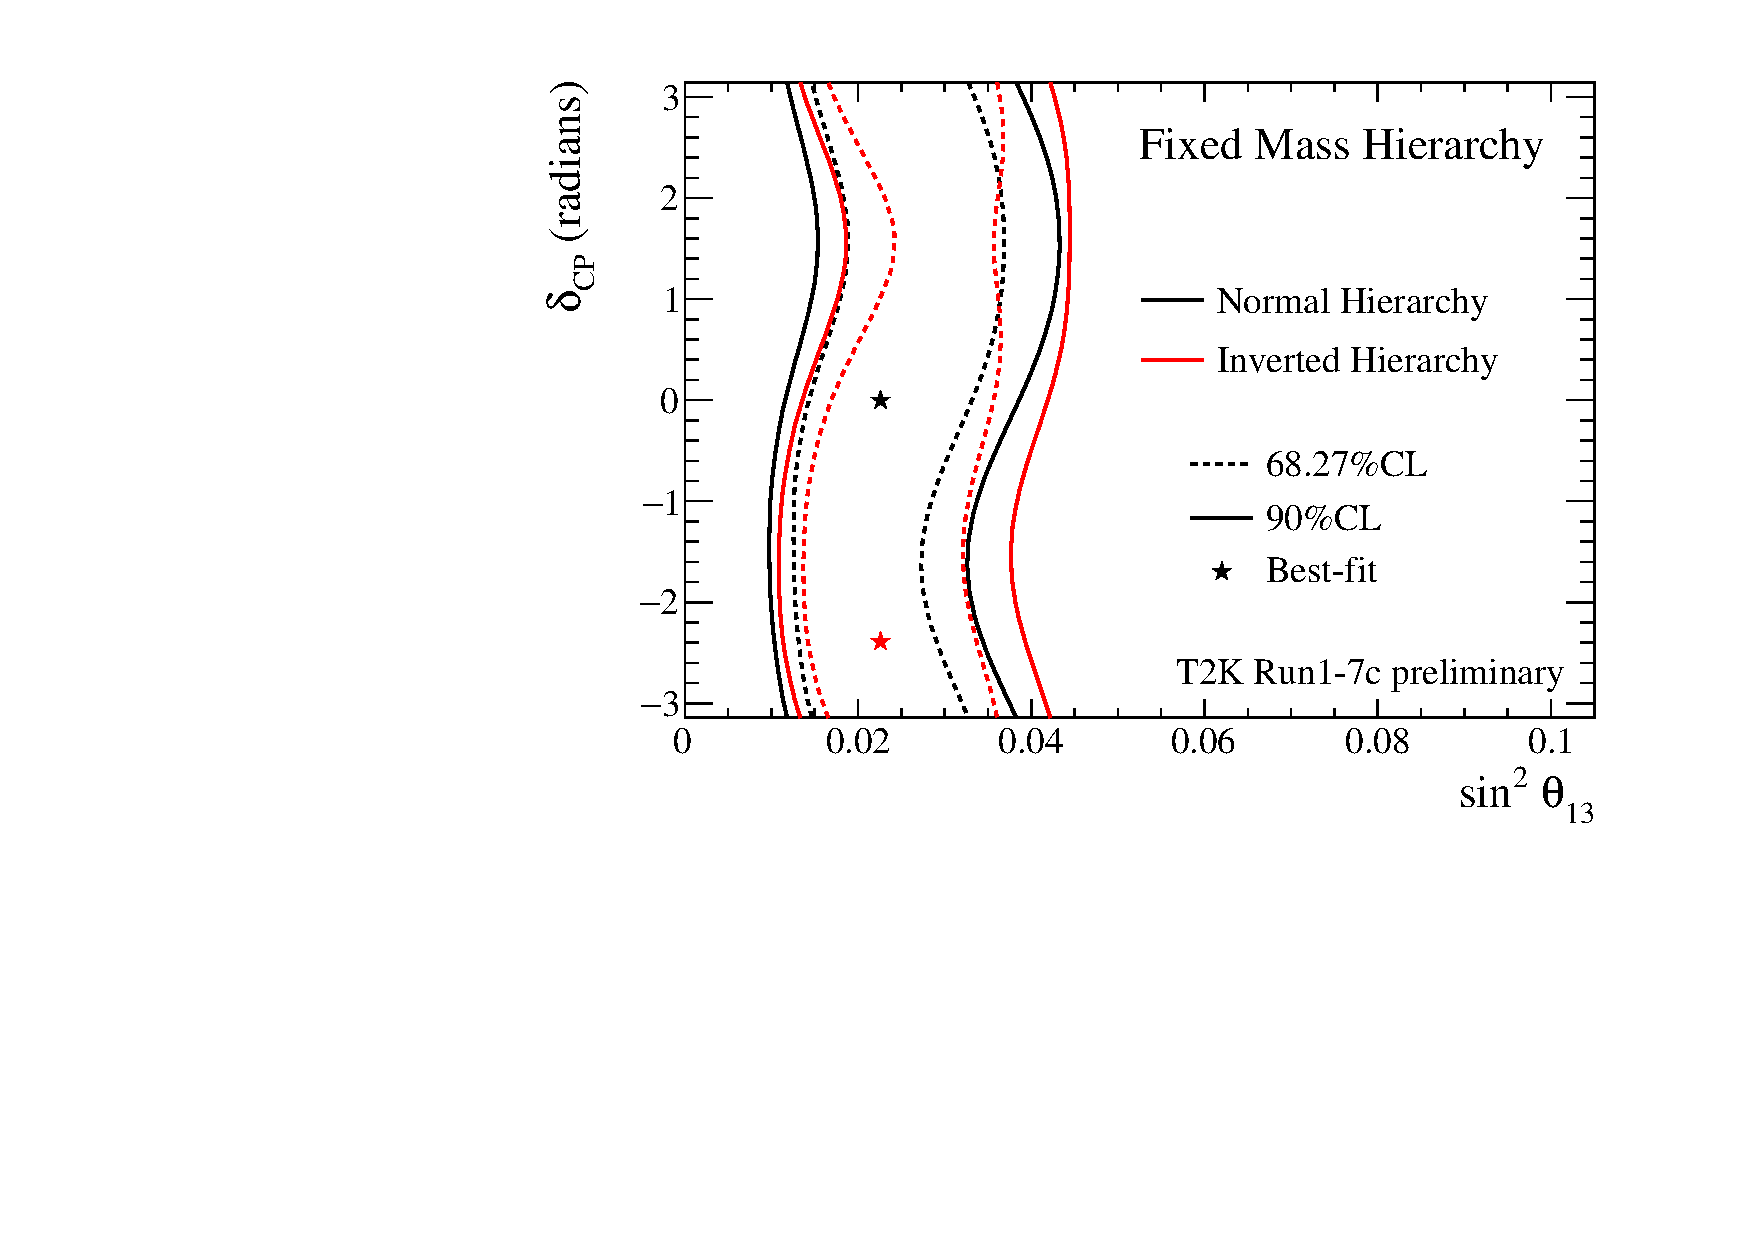
\includegraphics[width=0.9\textwidth]{./joint_plots/sensitivities/CDE/C_dcp_ss13_t2konly.pdf}
\caption{Asimov C: $\sin^2 \theta_{13}$ Vs $\delta_{CP}$.}
\end{subfigure}
\begin{subfigure}[b]{0.49\textwidth}
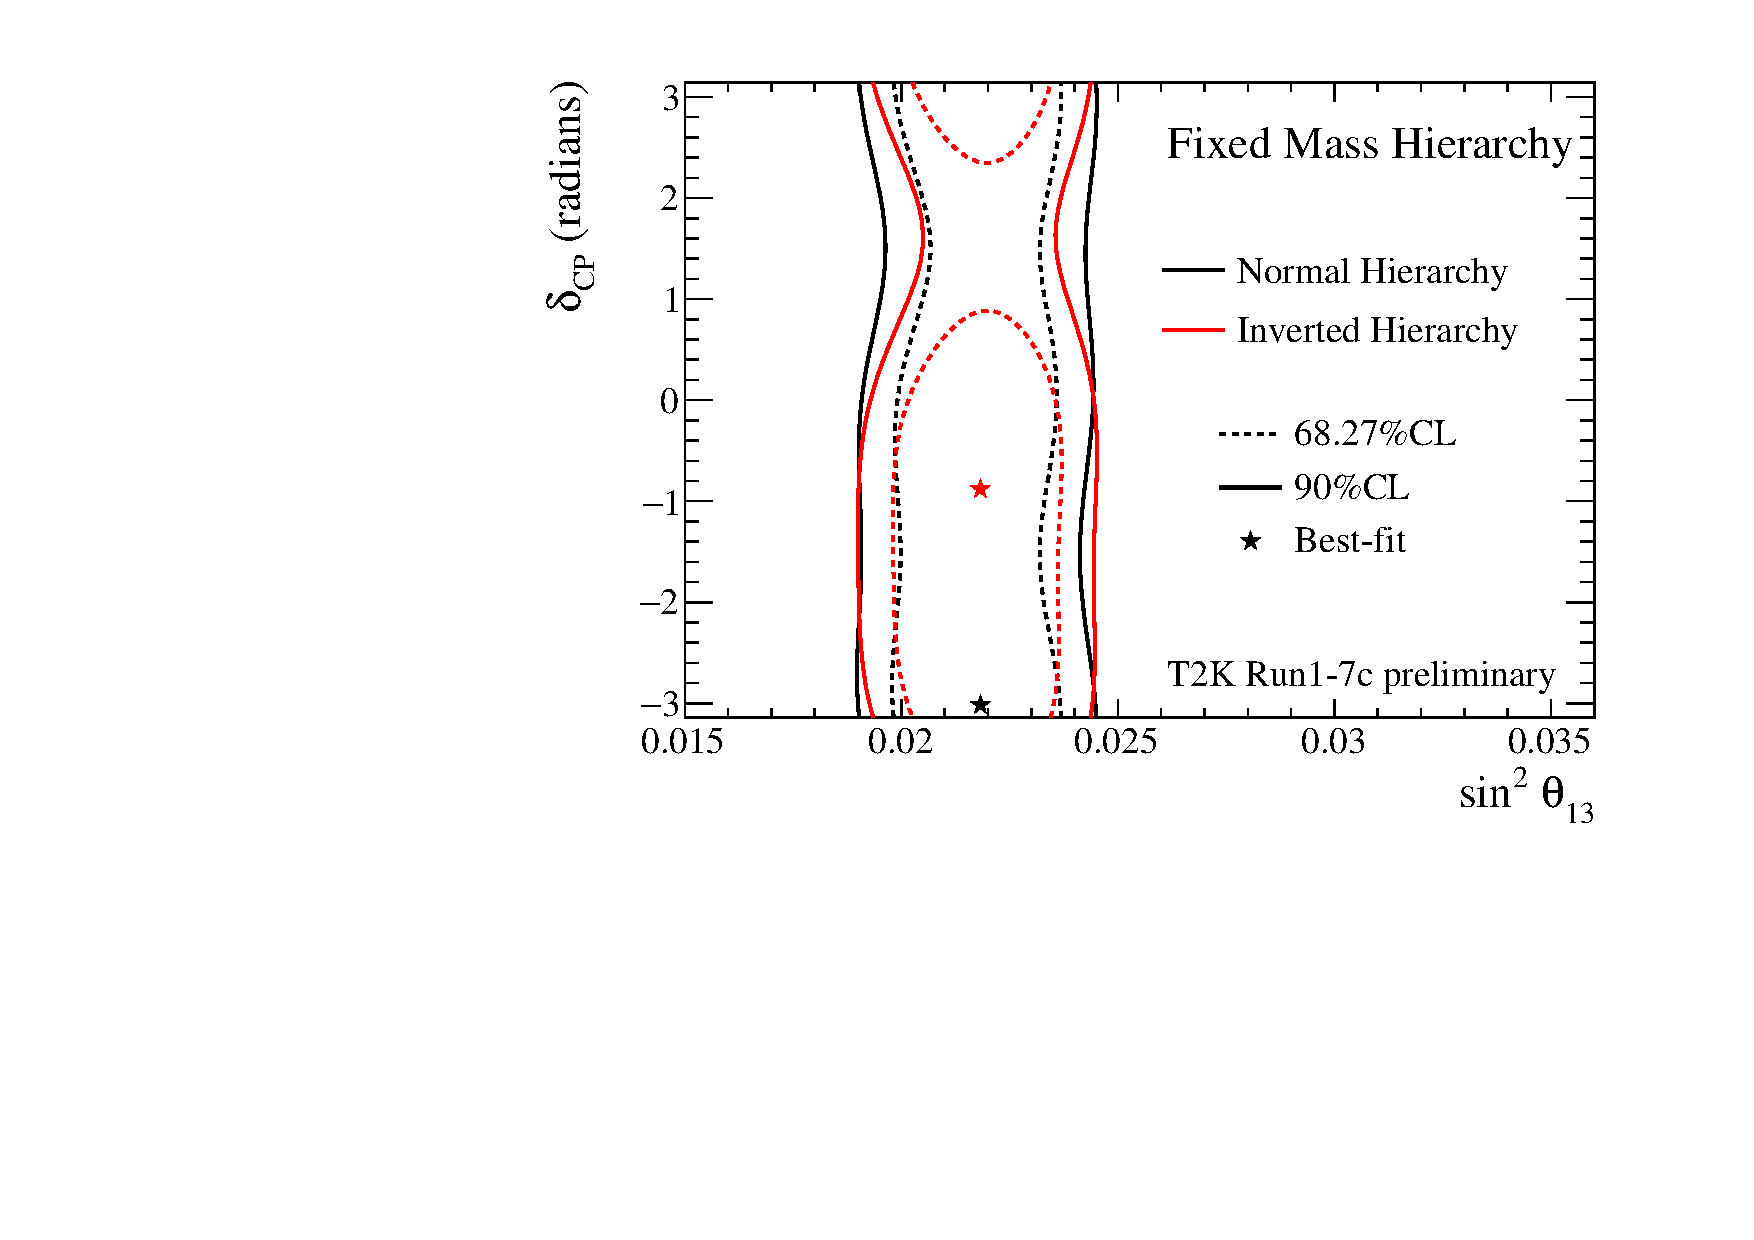
\includegraphics[width=0.9\textwidth]{./joint_plots/sensitivities/CDE/D_dcp_ss13_reactor.pdf}
\caption{Asimov D: $\sin^2 \theta_{13}$ Vs $\delta_{CP}$. Reactor constraint.}
\end{subfigure}
\begin{subfigure}[b]{0.49\textwidth}
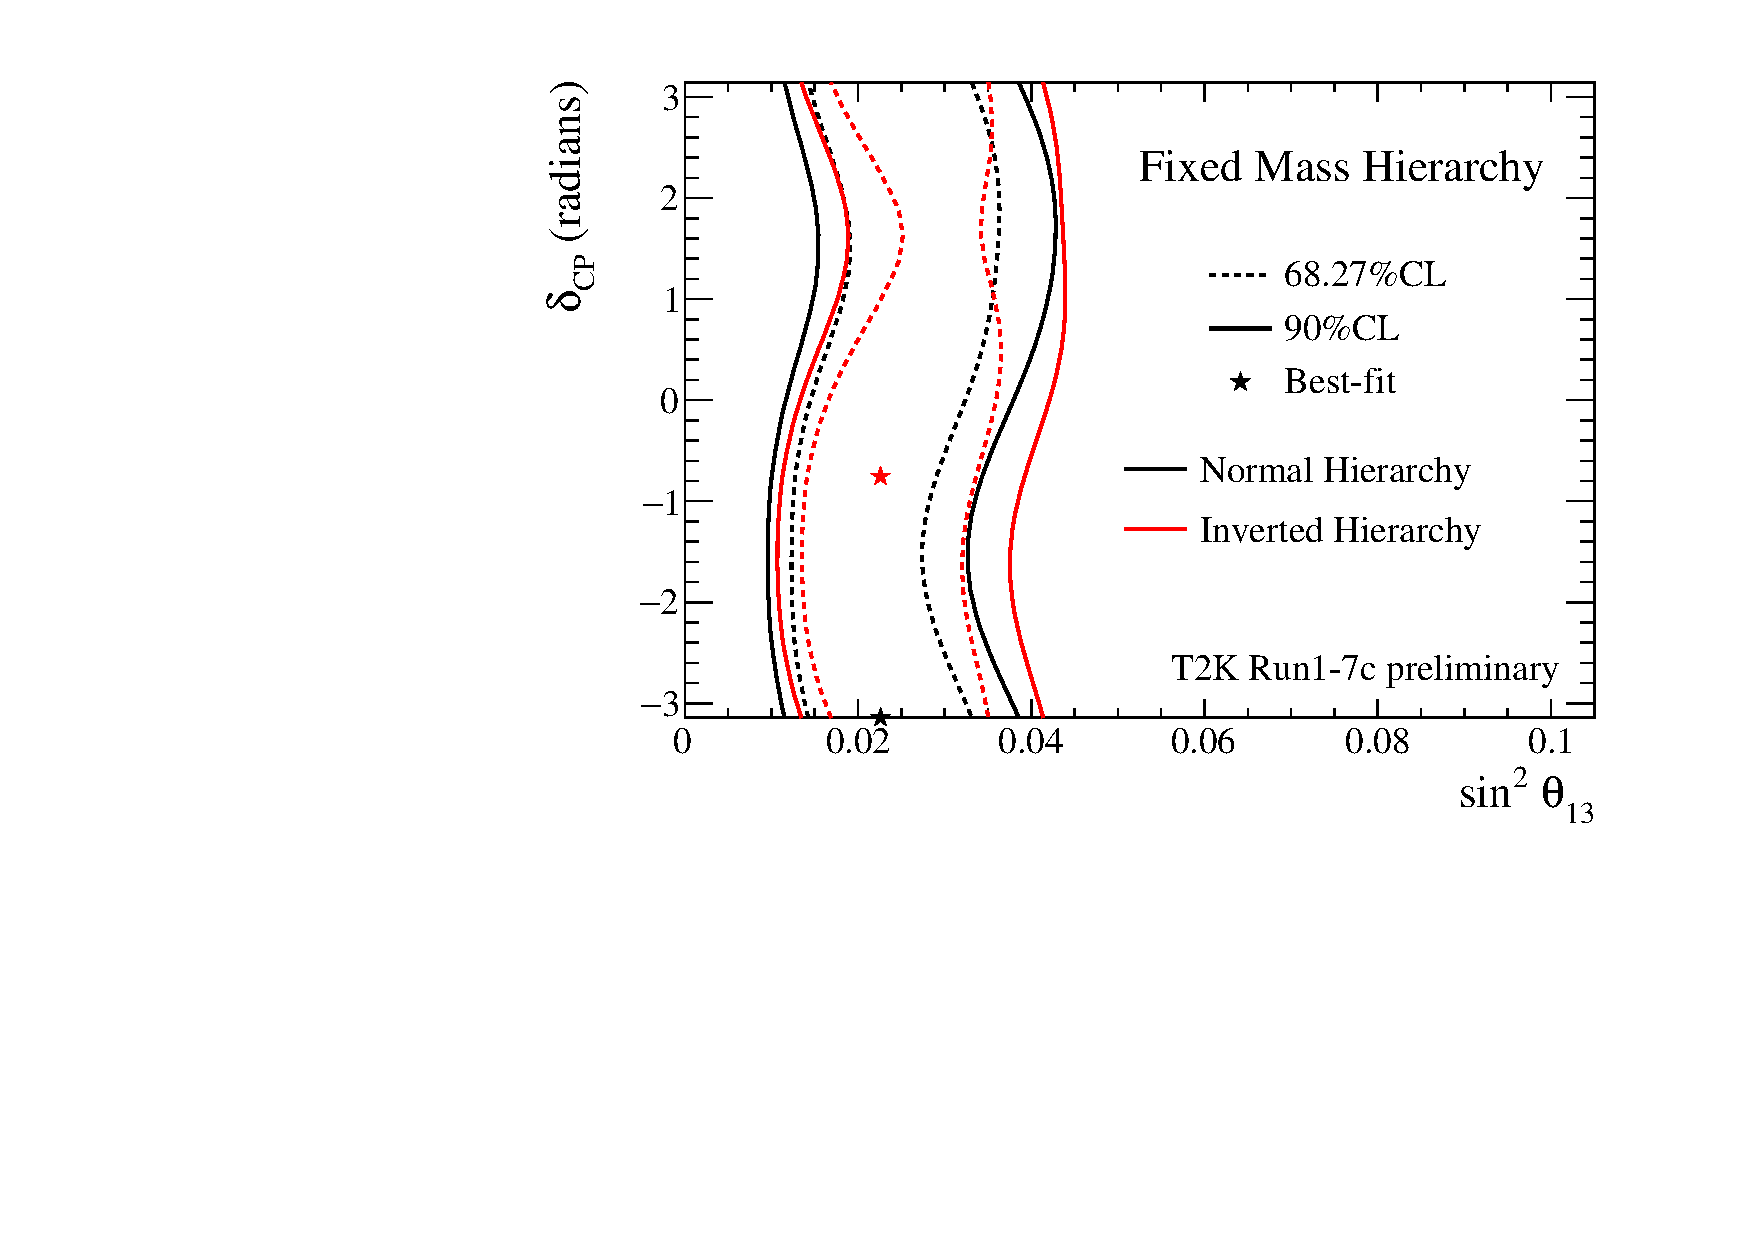
\includegraphics[width=0.9\textwidth]{./joint_plots/sensitivities/CDE/D_dcp_ss13_t2konly.pdf}
\caption{Asimov D: $\sin^2 \theta_{13}$ Vs $\delta_{CP}$.}
\end{subfigure}
\begin{subfigure}[b]{0.49\textwidth}
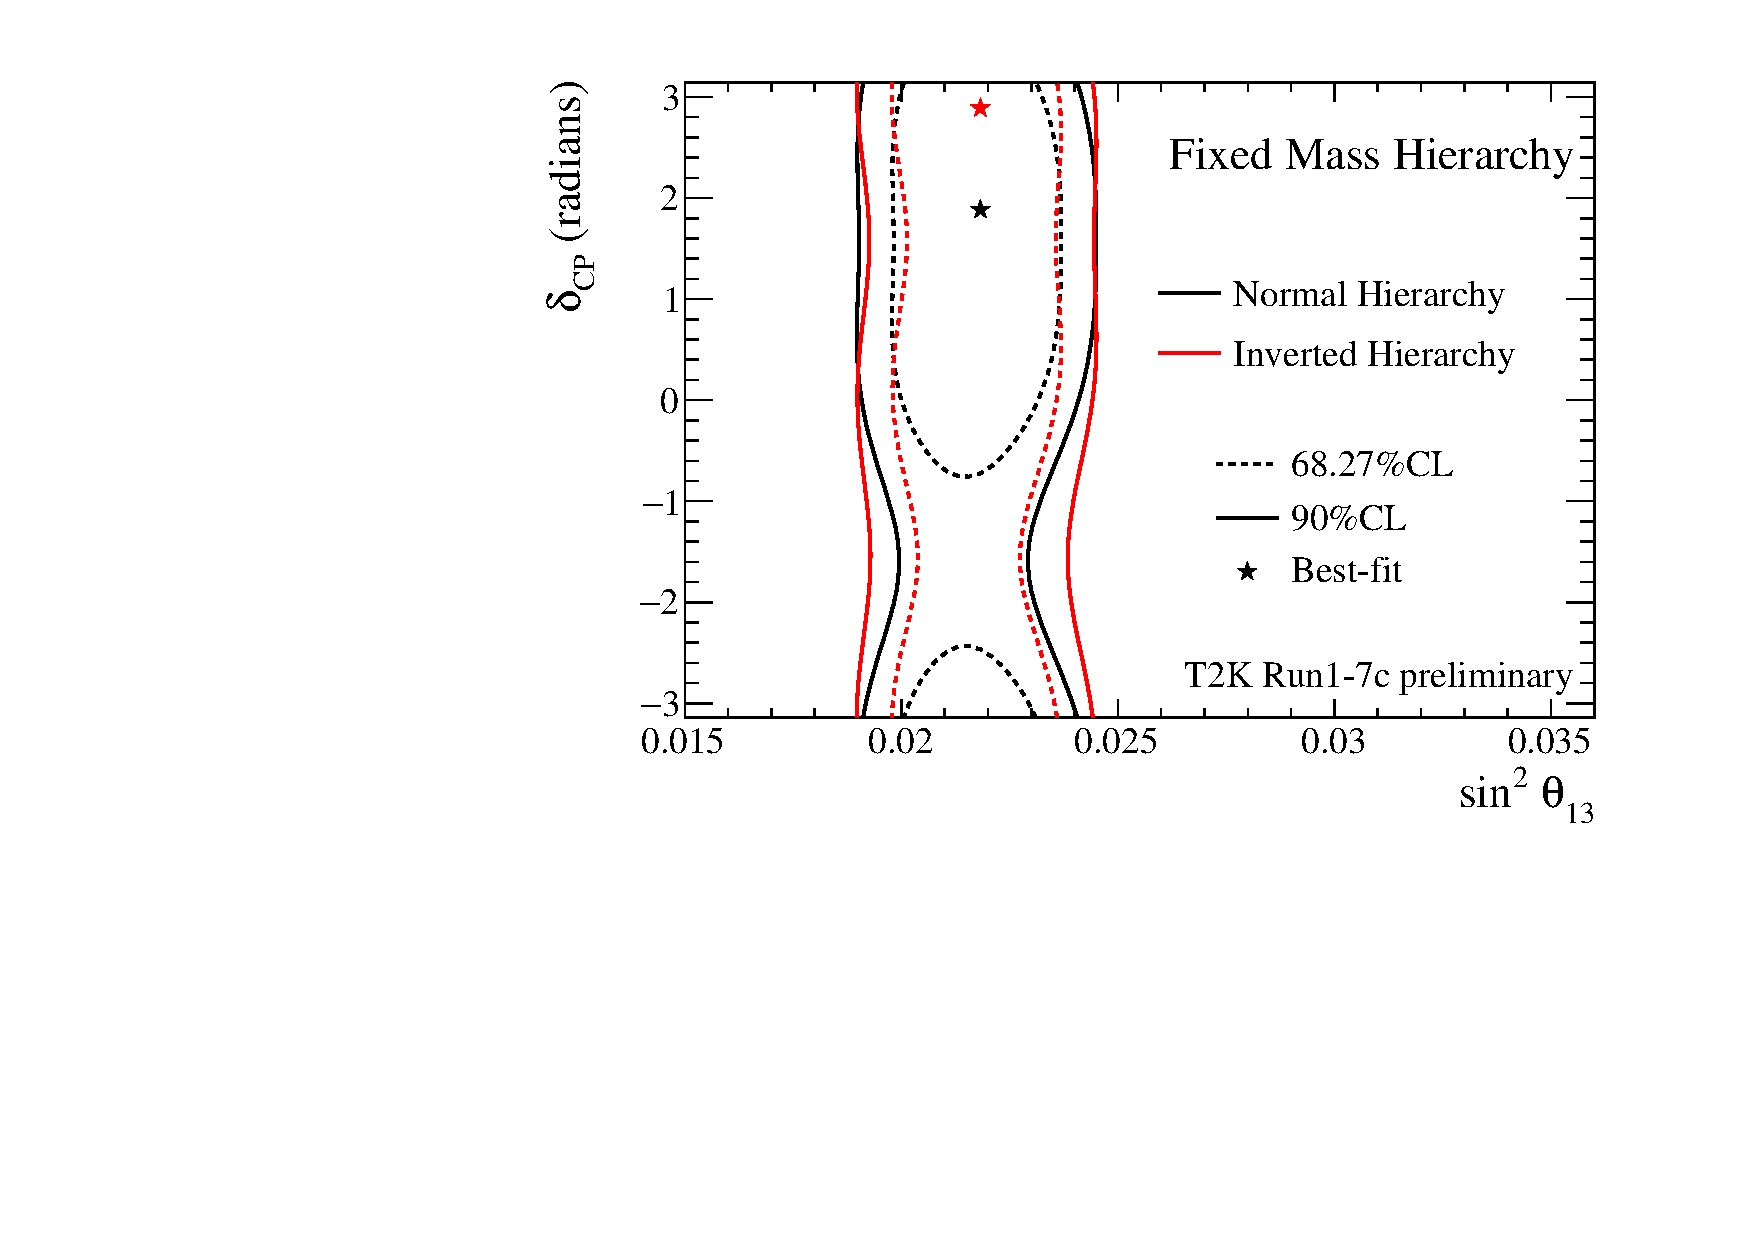
\includegraphics[width=0.9\textwidth]{./joint_plots/sensitivities/CDE/E_dcp_ss13_reactor.pdf}
\caption{Asimov E: $\sin^2 \theta_{13}$ Vs $\delta_{CP}$. Reactor constraint.}
\end{subfigure}
\begin{subfigure}[b]{0.49\textwidth}
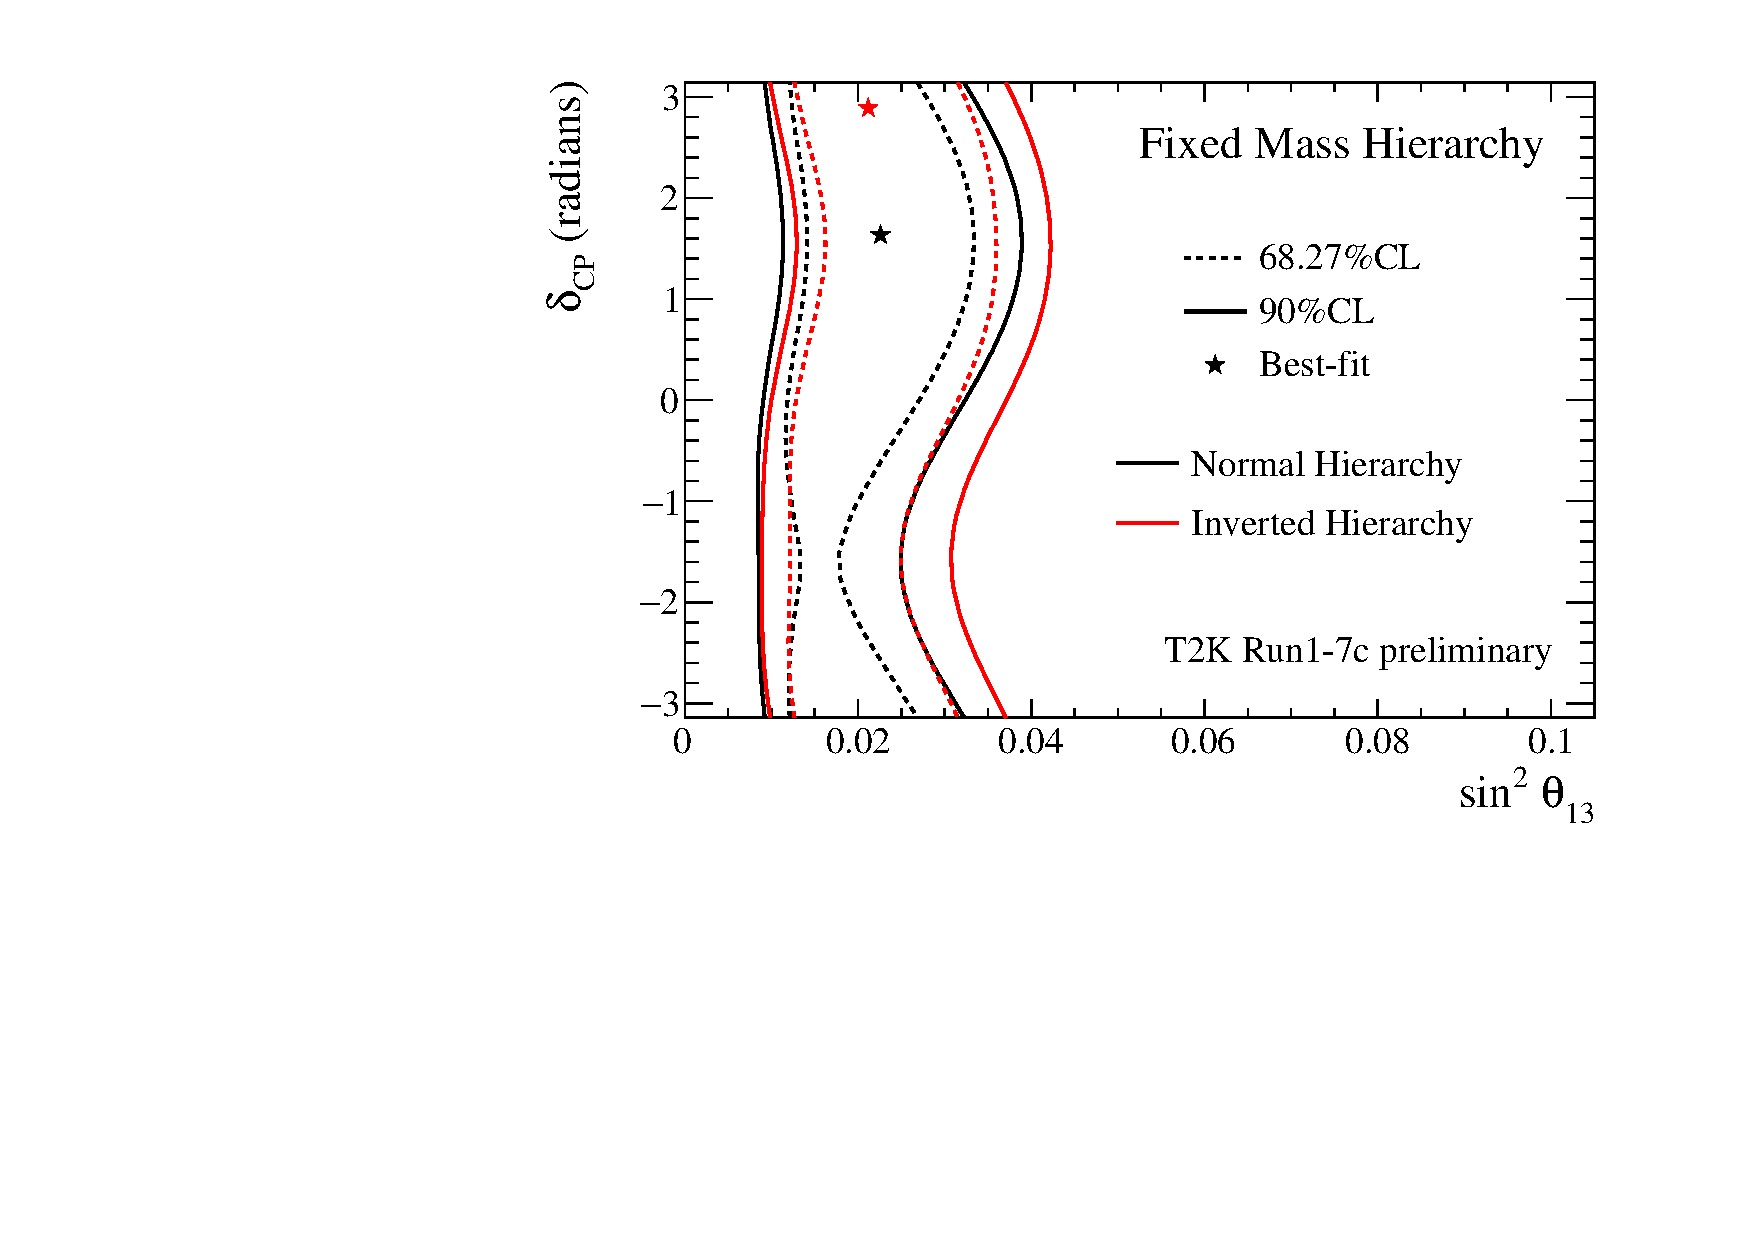
\includegraphics[width=0.9\textwidth]{./joint_plots/sensitivities/CDE/E_dcp_ss13_t2konly.pdf}
\caption{Asimov E: $\sin^2 \theta_{13}$ Vs $\delta_{CP}$.}
\end{subfigure}
\caption {
%{\large{SENSI 2D CONTOURS W/ AND W/O REACTORS}}
The contours at 68\% and 90\% CL with reactor constraint 
for the Asimov data sets C, D and E of \cref{tab:osc_params_joint_asimov} 
corresponding to the Run 1-7c statistics 
is shown.
%is compared to the result obtained by the other analysis groups.
Normal and inverted hierarchy contours are independent.
}
\label{fig:validation_sensi_2d_reactors_cde}
\end{figure*}

\begin{figure*}[htb]
\center
\begin{subfigure}[b]{0.49\textwidth}
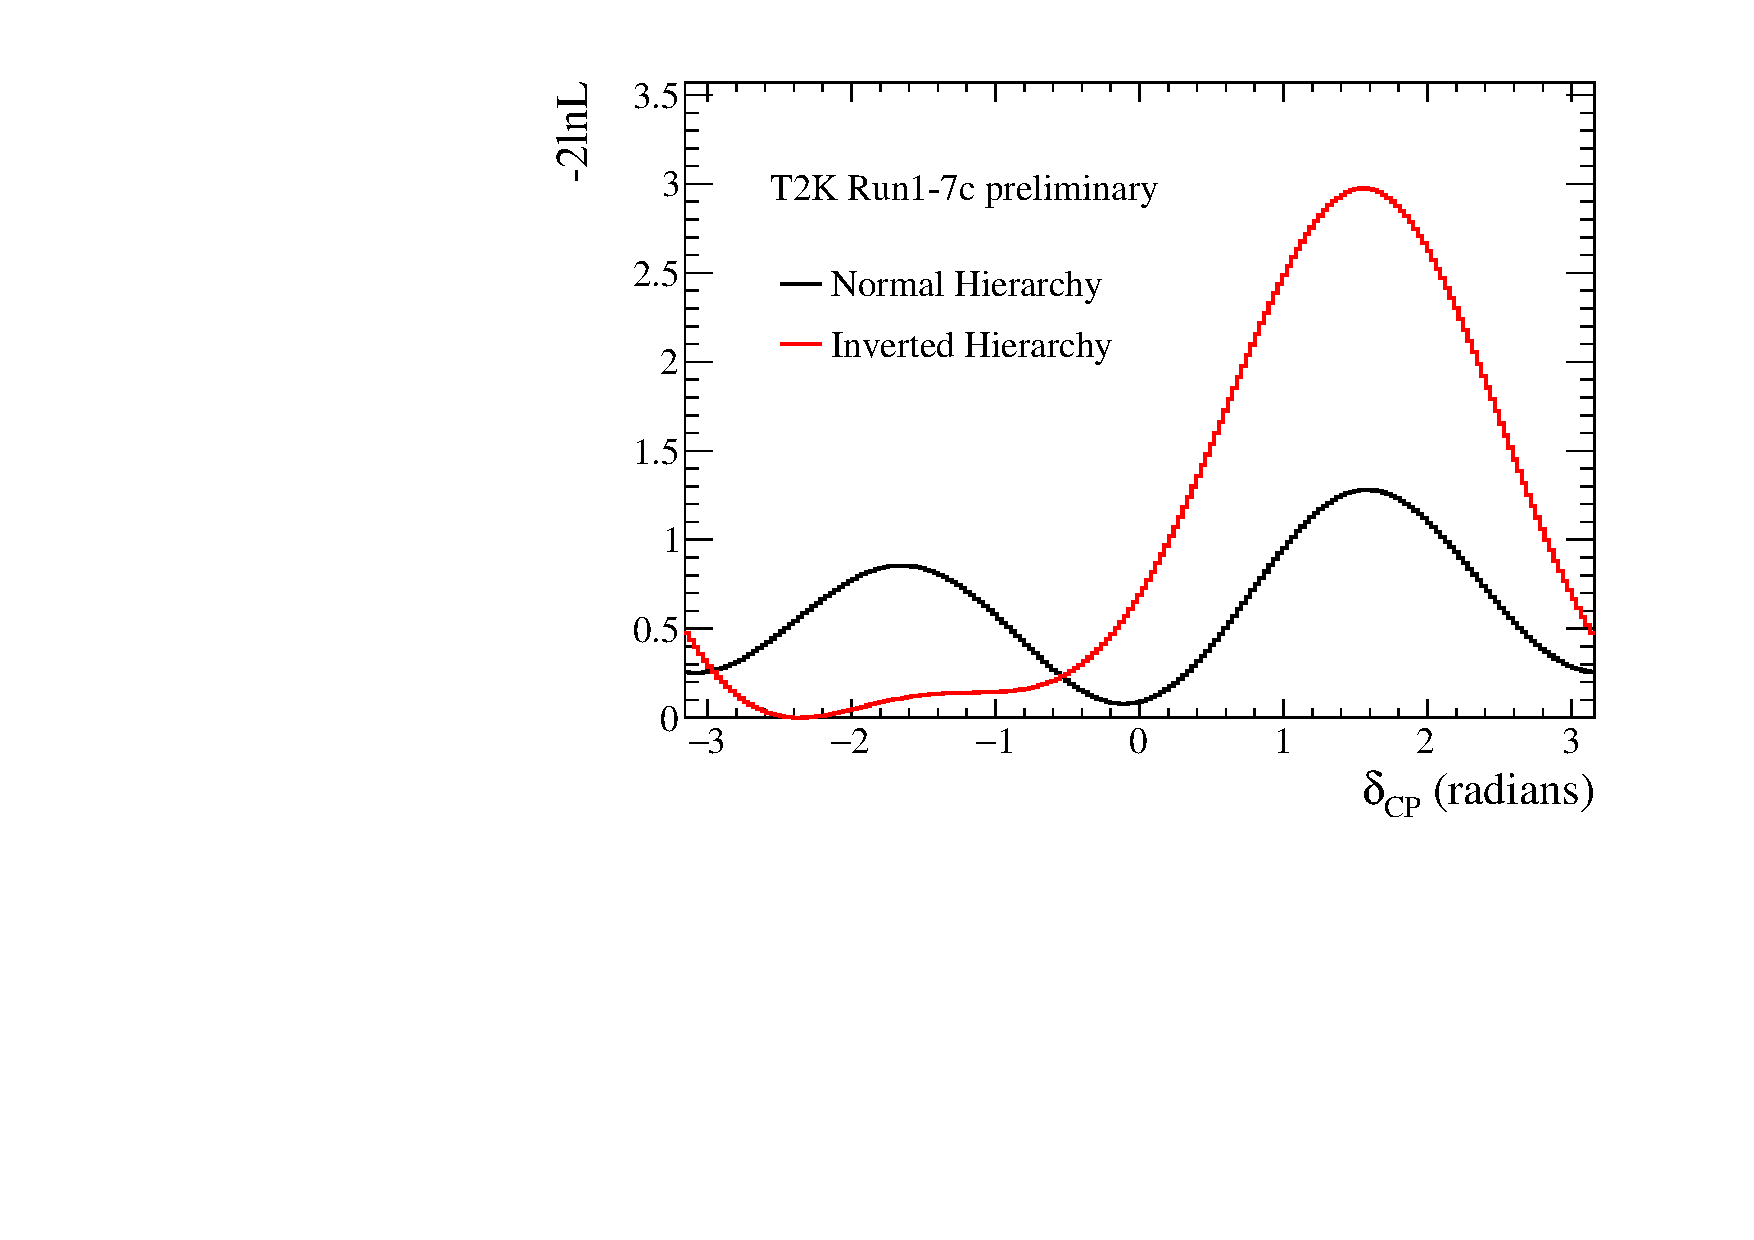
\includegraphics[width=0.9\textwidth]{./joint_plots/sensitivities/CDE/C_dcp_reactor.pdf}
\caption{Asimov C}
\end{subfigure}
\begin{subfigure}[b]{0.49\textwidth}
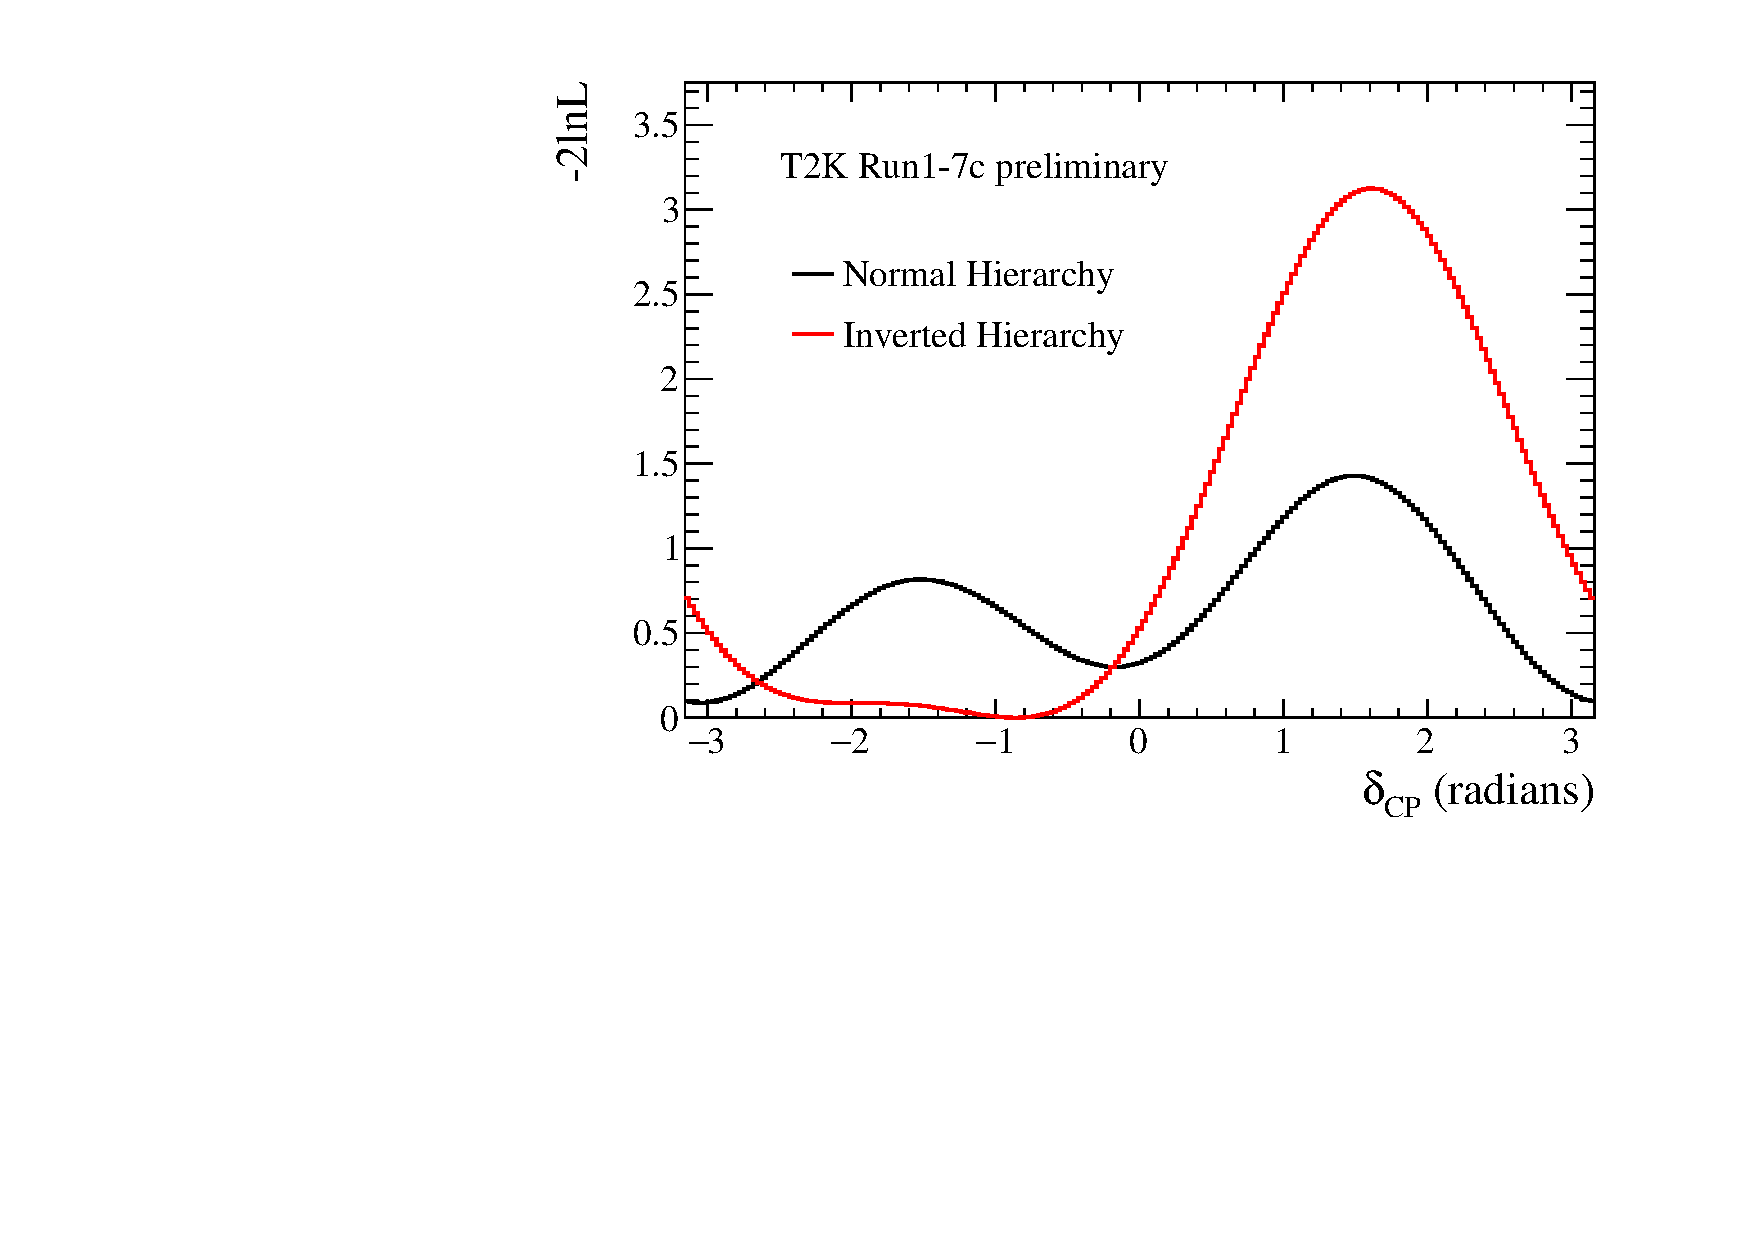
\includegraphics[width=0.9\textwidth]{./joint_plots/sensitivities/CDE/D_dcp_reactor.pdf}
\caption{Asimov D}
\end{subfigure}
\begin{subfigure}[b]{0.49\textwidth}
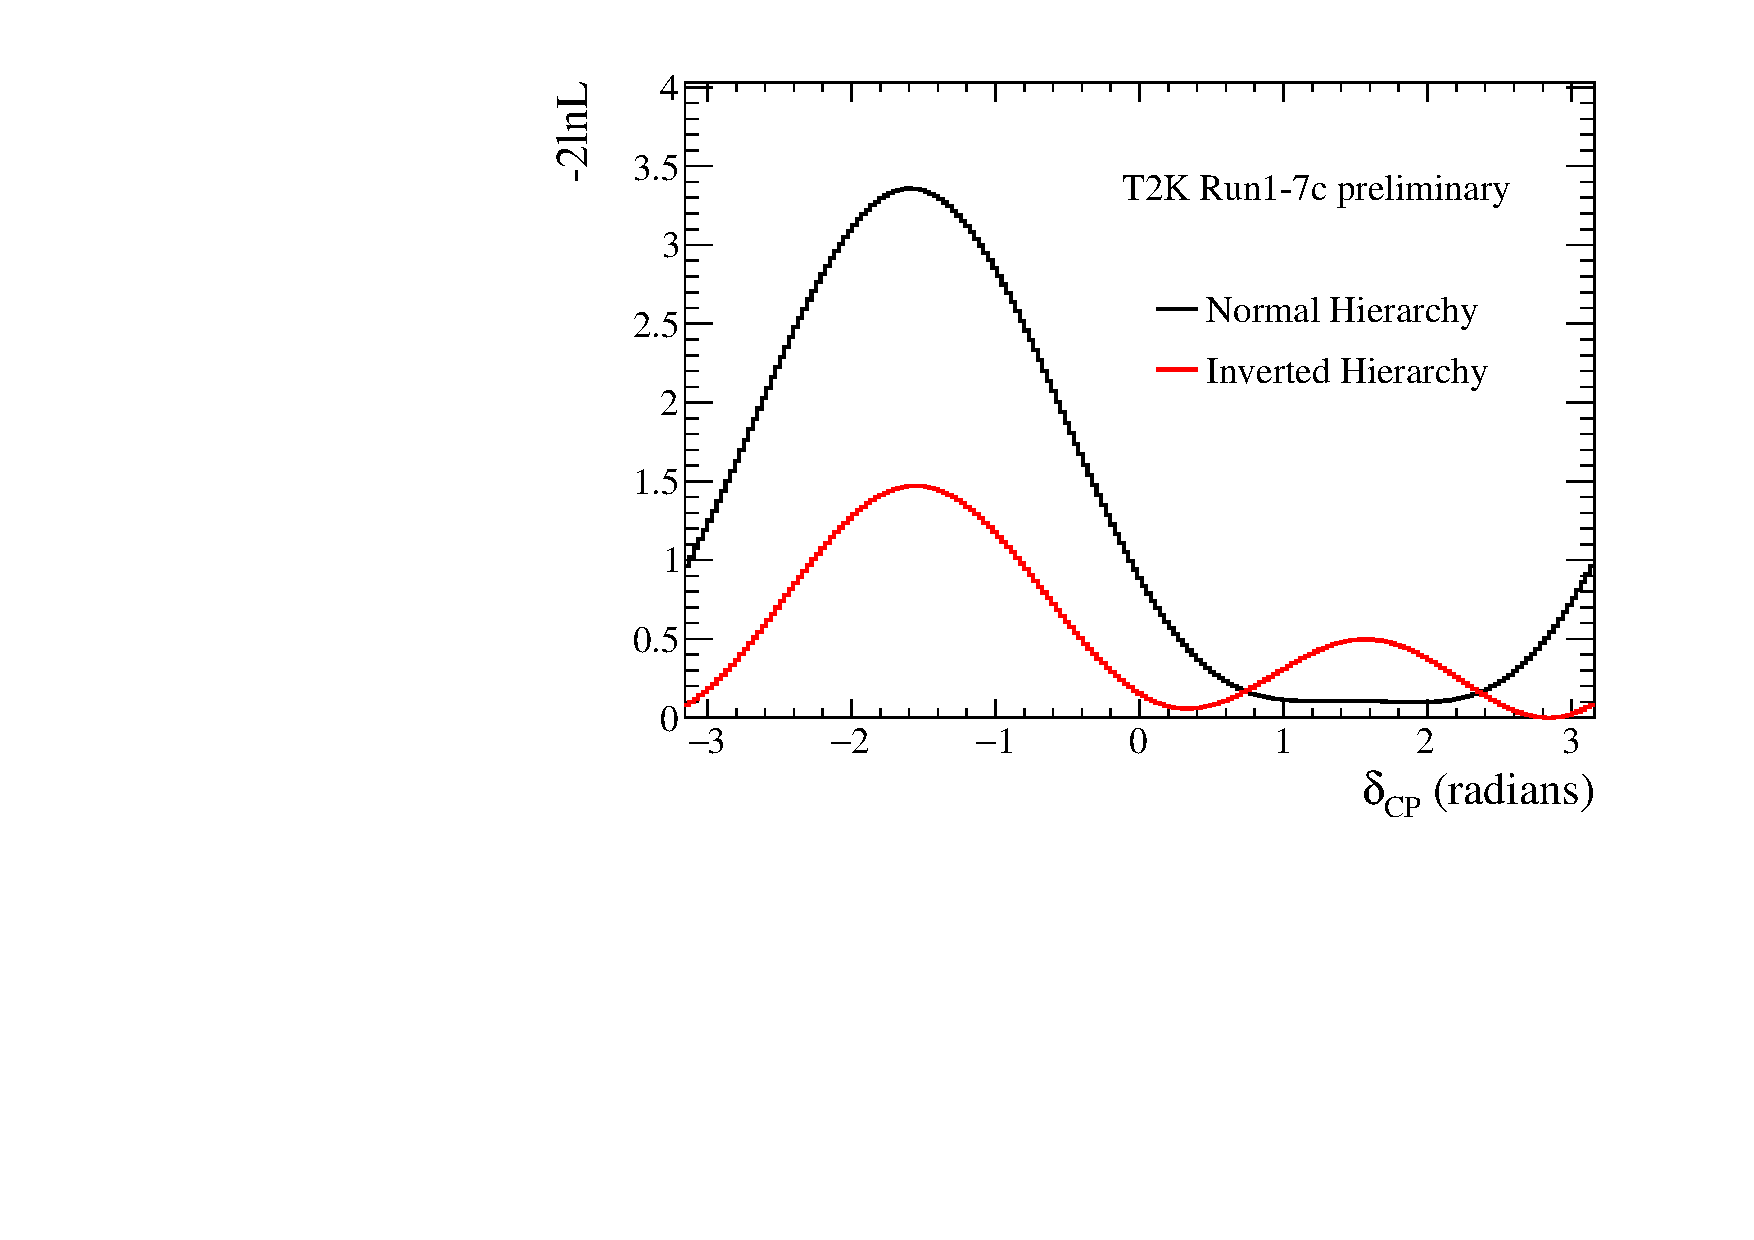
\includegraphics[width=0.9\textwidth]{./joint_plots/sensitivities/CDE/E_dcp_reactor.pdf}
\caption{Asimov E}
\end{subfigure}
%\begin{subfigure}[b]{0.49\textwidth}
%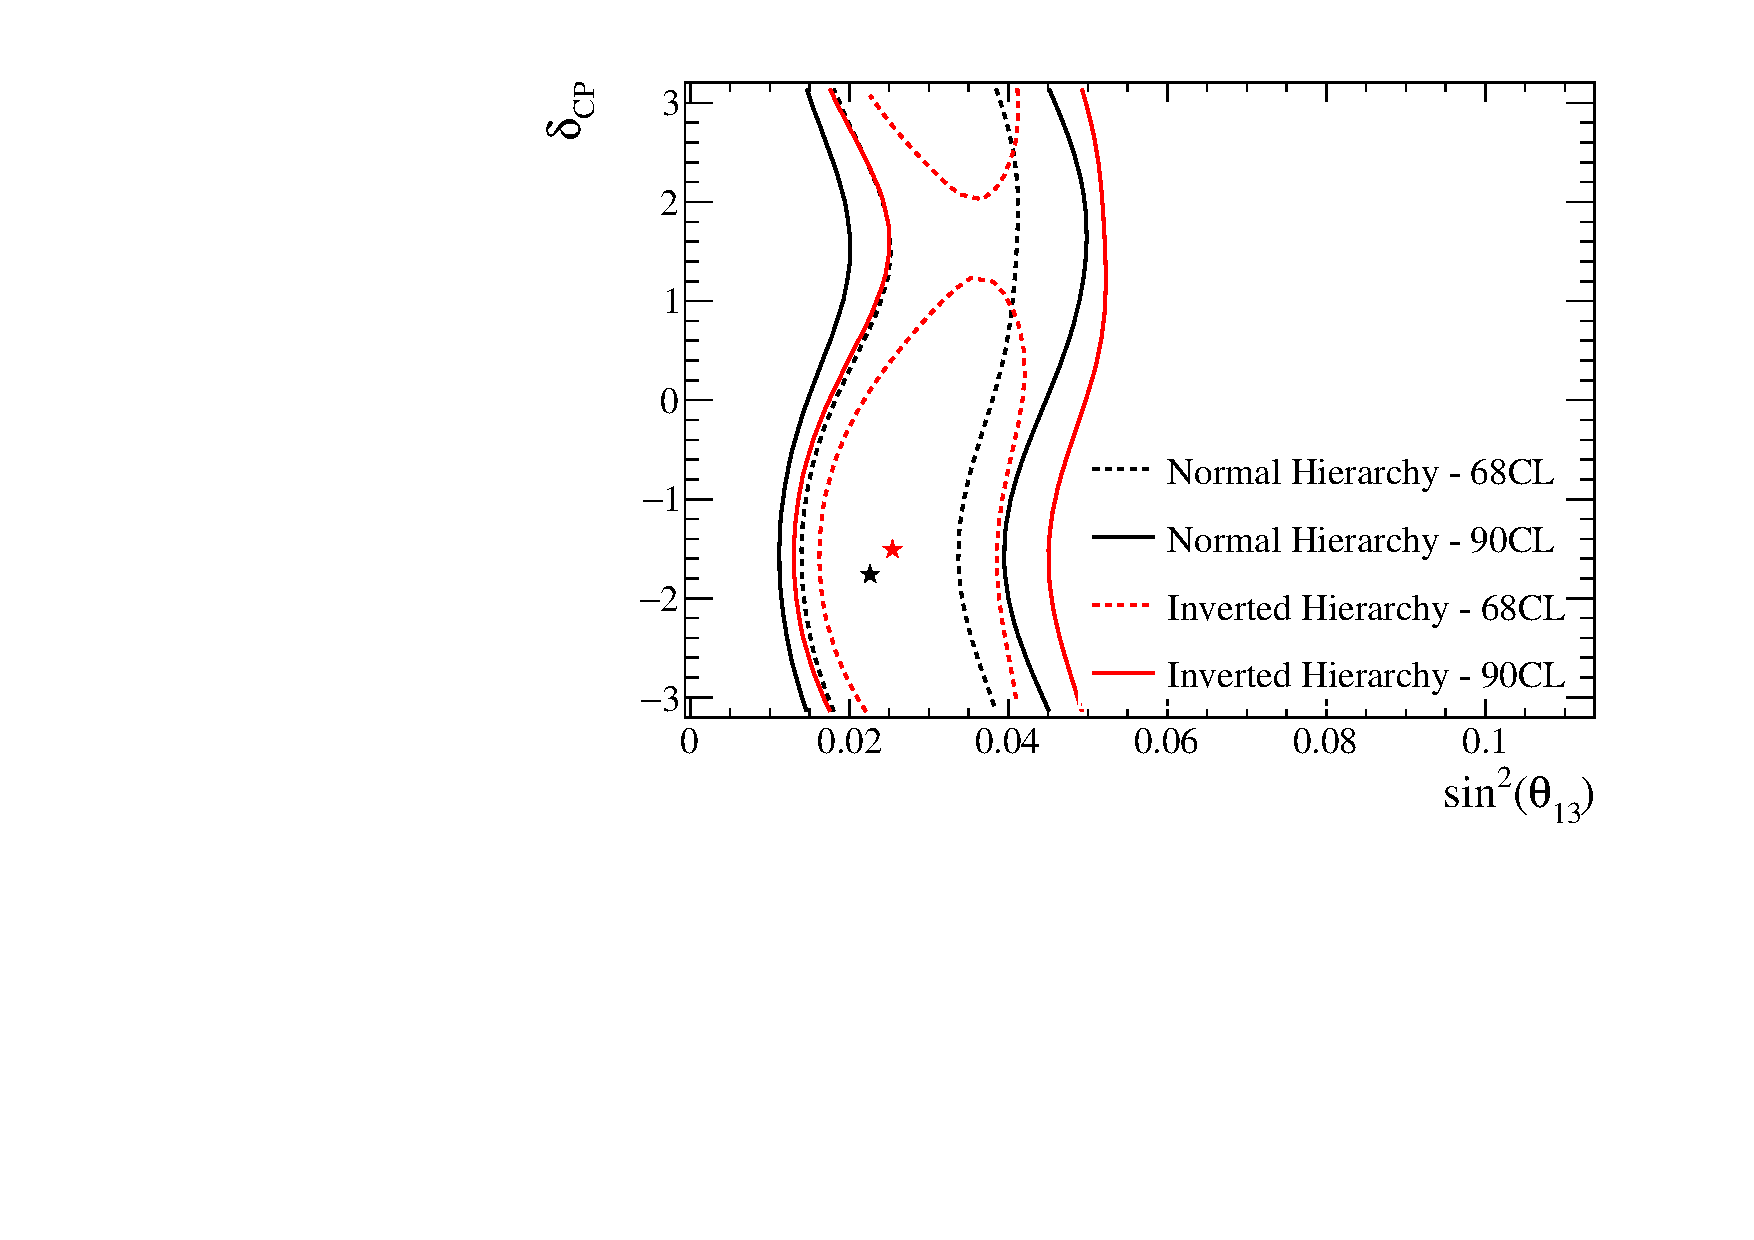
\includegraphics[width=0.9\textwidth]{./joint_plots/sensitivities/2D/cp13/cp13_A.pdf}
%\caption{Asimov A T2K only}
%\end{subfigure}
%\begin{subfigure}[b]{0.49\textwidth}
%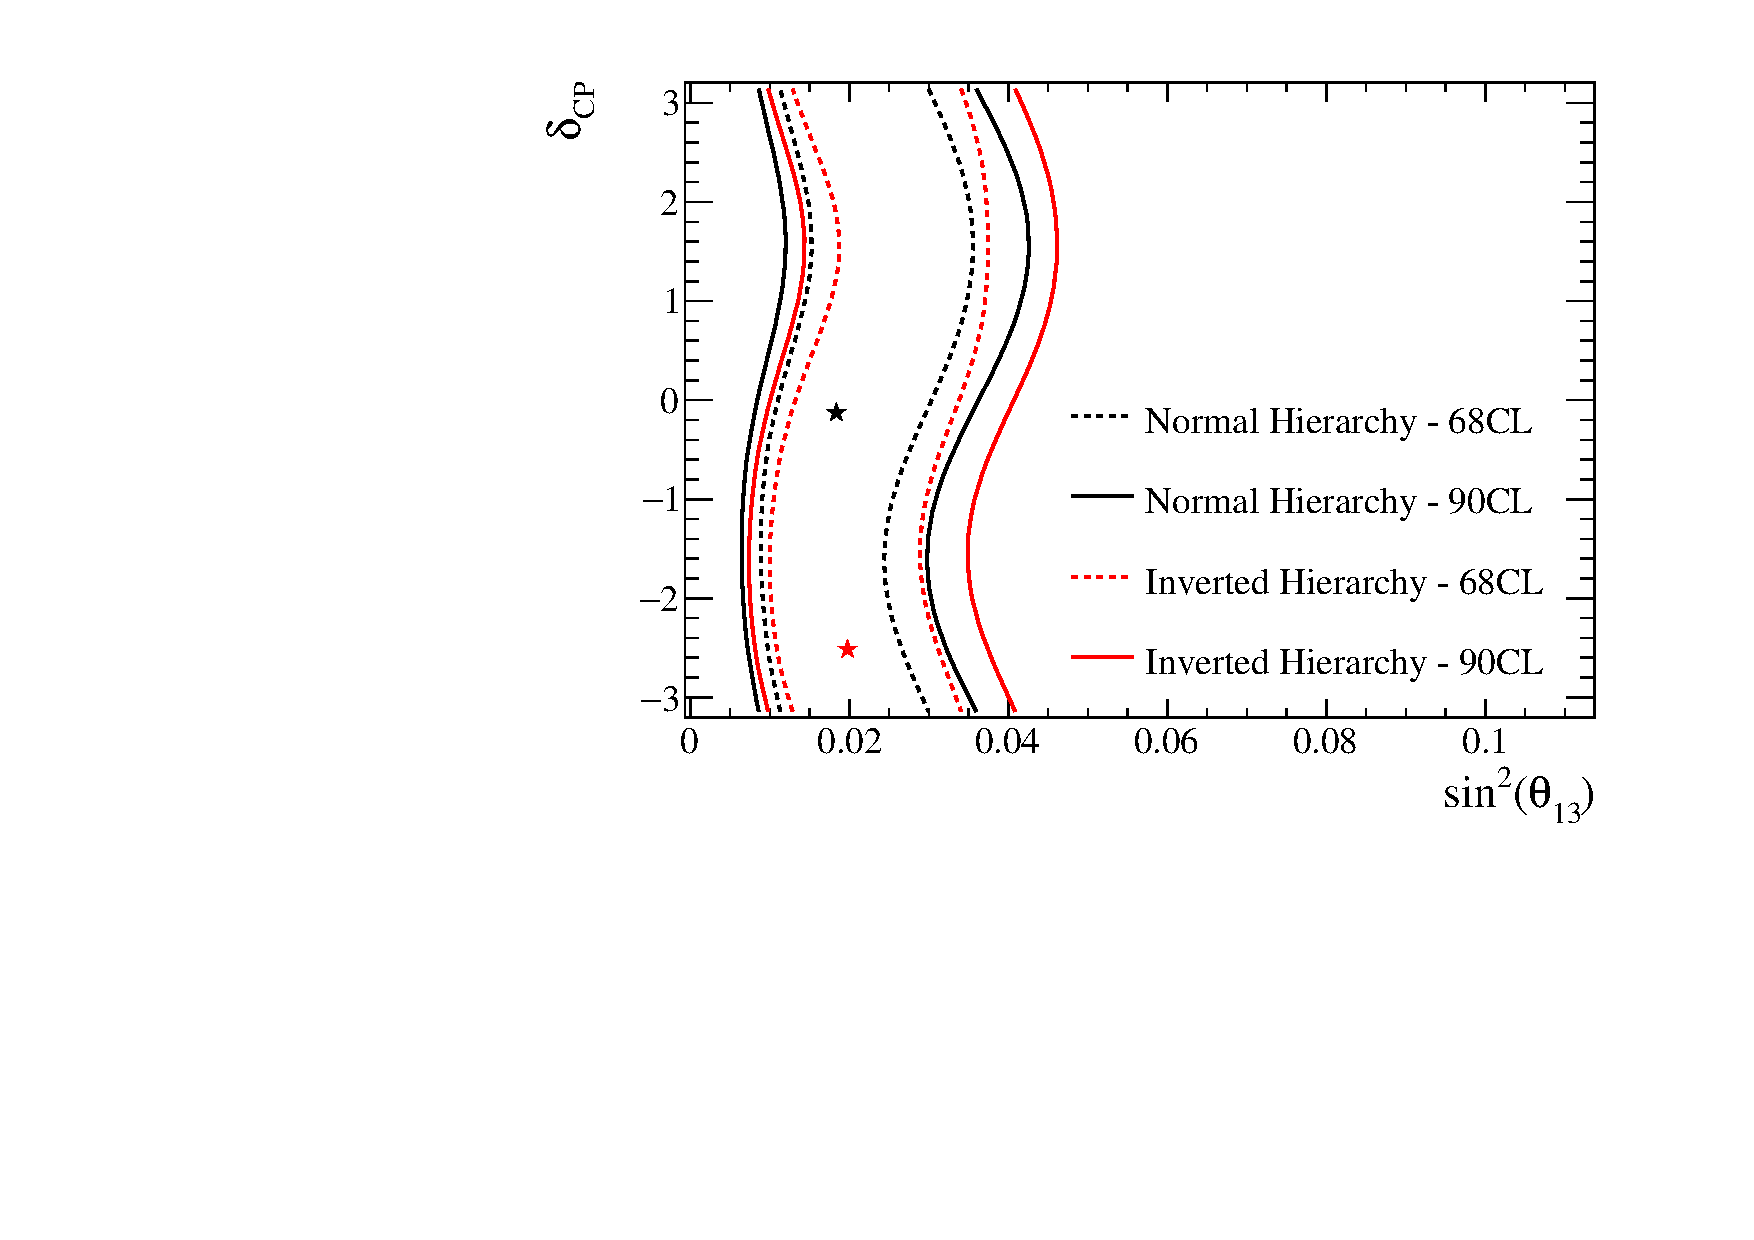
\includegraphics[width=0.9\textwidth]{./joint_plots/sensitivities/2D/cp13/cp13_B.pdf}
%\caption{Asimov B T2K only}
%\end{subfigure}

%\includegraphics[width=0.9\textwidth]{./joint_plots/sensitivities/2D/}
%\includegraphics[width=0.9\textwidth]{./joint_plots/sensitivities/2D/} \\
%\includegraphics[width=0.9\textwidth]{./joint_plots/sensitivities/2D/}
%\includegraphics[width=0.9\textwidth]{./joint_plots/sensitivities/2D/}
\caption {
%{\large{SENSI 2D CONTOURS W/ AND W/O REACTORS}}
The contours 1D $\delta_{CP}$ contours 
for the Asimov data sets C, D and E of \cref{tab:osc_params_joint_asimov} 
with the reactor constraint
corresponding to the Run 1-7c statistics 
is shown.
%is compared to the result obtained by the other analysis groups.
Normal and inverted hierarchy contours are independent.
}
\label{fig:validation_sensi_dcp_cde}
\end{figure*}

%In Fig.~\ref{fig:validation_data_Run14_1d} and~\ref{fig:validation_data_run14_2d} 
%the same $\Delta \chi^2$ distributions for $\delta_{CP}$ 
%as well as the same contours are 
%shown for the Run 1-4 data set and compared to the other analysis groups results.
%
%\begin{figure*}[htb]
%\center
%
\includegraphics[width=0.9\textwidth]{./images/missing_plot-eps-converted-to.pdf}
%
\includegraphics[width=0.9\textwidth]{./images/missing_plot-eps-converted-to.pdf}
%\caption {
%{\large{RUN14 DELTACHISQ 1D DELTACP W/ AND W/O REACTORS}}
%The $\Delta \chi^2$ distribution as a function of $\delta_{CP}$ 
%with reactor constraint (left) and T2K only data (right) 
%for the Run 1-4 data set
%is compared to the result obtained by the other analysis groups.
%The mass hierarchy is minimized:
%both the normal and inverted hierarchy $\chi^2$ distributions 
%are shifted to the same global best-fit $\chi^2$ value,
%which is taken as the minimum between normal and inverted hierarchy.
%}
%\label{fig:validation_data_run14_1d}
%\end{figure*}
%
%\begin{figure*}[htb]
%\center
%
\includegraphics[width=0.9\textwidth]{./images/missing_plot-eps-converted-to.pdf}
%
\includegraphics[width=0.9\textwidth]{./images/missing_plot-eps-converted-to.pdf}
%
\includegraphics[width=0.9\textwidth]{./images/missing_plot-eps-converted-to.pdf}
%\caption {
%{\large{RUN14 2D CONTOURS W/ AND W/O REACTORS}}
%The contours at 68\% and 90\% CL 
%of $\sin^2 \theta_{13}$ Vs $\delta_{CP}$ 
%with reactor constraint (top left) and T2K only data (top right)
%and
%$\sin^2 \theta_{23}$ Vs $|\Delta m^2_{32}|$ 
%with reactor constraint (bottom left) and T2K only data (bottom right)
%for the Run 1-4 data set of tab.~\ref{tab:osc_params_joint} 
%is compared to the result obtained by the other analysis groups.
%Normal and inverted hierarchy contours are independent.
%}
%\label{fig:validation_data_run14_2d}
%\end{figure*}
%
%\vspace{3mm}
%{\huge{
%TODO: ADD COMMENT ON THE SENSITIVITY COMPARISONS
%}}
%\vspace{3mm}

